\documentclass[10pt,letterpaper]{article}
\usepackage[top=0.85in,left=2.75in,footskip=0.75in]{geometry}

% amsmath and amssymb packages, useful for mathematical formulas and symbols
\usepackage{amsmath,amssymb}

% Use adjustwidth environment to exceed column width (see example table in text)
\usepackage{changepage}

% Use Unicode characters when possible
\usepackage[utf8x]{inputenc}

% textcomp package and marvosym package for additional characters
\usepackage{textcomp,marvosym}

% cite package, to clean up citations in the main text. Do not remove.
\usepackage{cite}

% Use nameref to cite supporting information files (see Supporting Information section for more info)
\usepackage{nameref,hyperref}

% line numbers
\usepackage[right]{lineno}

% ligatures disabled
\usepackage{microtype}
\DisableLigatures[f]{encoding = *, family = * }

% color can be used to apply background shading to table cells only
\usepackage[table]{xcolor}

% array package and thick rules for tables
\usepackage{array}

% enumerate package lets us use letters instead of numbers
\usepackage{enumerate}

% create "+" rule type for thick vertical lines
\newcolumntype{+}{!{\vrule width 2pt}}

% create \thickcline for thick horizontal lines of variable length
\newlength\savedwidth
\newcommand\thickcline[1]{%
  \noalign{\global\savedwidth\arrayrulewidth\global\arrayrulewidth 2pt}%
  \cline{#1}%
  \noalign{\vskip\arrayrulewidth}%
  \noalign{\global\arrayrulewidth\savedwidth}%
}

% \thickhline command for thick horizontal lines that span the table
\newcommand\thickhline{\noalign{\global\savedwidth\arrayrulewidth\global\arrayrulewidth 2pt}%
\hline
\noalign{\global\arrayrulewidth\savedwidth}}

\usepackage{color}

% Remove comment for double spacing
%\usepackage{setspace}
%\doublespacing

% Text layout
\raggedright
\setlength{\parindent}{0.5cm}
\textwidth 5.25in
\textheight 8.75in

% Bold the 'Figure #' in the caption and separate it from the title/caption with a period
% Captions will be left justified
\usepackage[aboveskip=1pt,labelfont=bf,labelsep=period,justification=raggedright,singlelinecheck=off]{caption}
\renewcommand{\figurename}{Fig}

% Use the PLoS provided BiBTeX style
\bibliographystyle{plos2015}

% Remove brackets from numbering in List of References
\makeatletter
\renewcommand{\@biblabel}[1]{\quad#1.}
\makeatother

% Leave date blank
\date{}

% Header and Footer with logo
\usepackage{lastpage,fancyhdr,graphicx}
\usepackage{epstopdf}
\pagestyle{myheadings}
\pagestyle{fancy}
\fancyhf{}
\setlength{\headheight}{27.023pt}
\lhead{
\includegraphics[width=2.0in]{PLOS-submission.eps}}
\rfoot{\thepage/\pageref{LastPage}}
\renewcommand{\footrule}{\hrule height 2pt \vspace{2mm}}
\fancyheadoffset[L]{2.25in}
\fancyfootoffset[L]{2.25in}
\lfoot{\sf PLOS}


%% Define per-paper macros.
\newcommand{\rulemajor}[1]{\section{#1}}
\begin{document}
\vspace*{0.2in}

\begin{flushleft}
{\Large
\textbf\newline{Ten Simple Rules for Helping Newcomers Become Contributors to Open Source Projects}
}
\newline
\\
{Mara Averick}\textsuperscript{1{\ddag}},
{Denae Ford}\textsuperscript{2{\ddag}},
{Mike Hoye}\textsuperscript{3{\ddag}},
{Jesse Mostipak}\textsuperscript{4{\ddag}},
{Dan Sholler}\textsuperscript{5{\ddag}},
{Greg~Wilson}\textsuperscript{1{\ddag}*}
\\
\bigskip
\textbf{1} RStudio, Inc. / \{mara.averick, greg.wilson\}@rstudio.com \\
\textbf{2} AFFILIATION / EMAIL \\
\textbf{3} AFFILIATION / EMAIL \\
\textbf{4} AFFILIATION / EMAIL \\
\bigskip
* Corresponding author. \\
\bigskip
{\ddag} These authors contributed equally to this work.
\end{flushleft}

\section*{Abstract}

FIXME: abstract.

\section*{Author Summary}

FIXME: one-paragraph summary.

\section*{Introduction}

According to \cite{b:wenger-cop}, communities of practice have three key characteristics:

\begin{enumerate}

\item participants have a common purpose or product that they work on or toward;

\item they are mutually engaged, i.e., they assist and mentor each another; and

\item they develop shared resources and domain knowledge.

\end{enumerate}

\rulemajor{Rule 1: Make governance explicit.}

Raymond's ``The Cathedral and the Bazaar'' (http://www.catb.org/esr/writings/cathedral-bazaar/)
was one of the most influential documents in the history of open source.
It described an egalitarian world in which everyone could contribute equally to the greater good,
but as Bezroukov pointed out in ``A Second Look at the Cathedral and the Bazaar'' (https://firstmonday.org/article/view/708/618),
that description ignored the realities of how power arises,
becomes concentrated in a few hands,
and is then used to perpetuate itself.
Bezroukov's criticism drew on Freeman's influential 1970 essay ``The Tyranny of Structurelessness'' (https://www.jofreeman.com/joreen/tyranny.htm),
which explained how an apparent lack of structure in organizations ``{\ldots}too often disguised an informal,
unacknowledged and unaccountable leadership that was all the more pernicious because its very existence was denied.''

Two decades later,
we can see how unequal and unwelcoming the supposedly egalitarian ``bazaar'' of open source can be
if authority lies with those willing to shout loudest and longest.
Making a project's governance explicit is therefore essential to making that project inviting and welcoming to newcomers with diverse backgrounds.
The most basic way to do this is to adopt something like the Contributor Covenant (https://www.contributor-covenant.org/),
which lays out groundrules for interpersonal interaction within the project.
At the opposite end,
large, well-established projects that incorporate as non-profits are required to promulgate bylaws,
such as those for the Python Software Foundation (https://www.python.org/psf/bylaws/).

What lies between these two extremes is less well documented,
but the ``Social and Political Infrastructure'' chapter of Fogel's \emph{Producing Open Source Software} (https://producingoss.com/en/producingoss.html)
is a good place to start.
It describes two models:

\begin{itemize}

\item
  A \emph{benevolent dictator} (who might better be called a ``community-approved arbitrator'') has final say,
  but their principal responsibility is to manage conversation to achieve consensus.

\item
  When consensus cannot be achieved,
  organizations may hold a vote.
  Organizations should decide who is and isn't eligible to vote well in advance of the emergence of issues requiring votes,
  since tempers may already been running hot by the time this point is reached.
  In the Carpentries (https://docs.carpentries.org/topic\_folders/governance/index.html),
  for example,
  anyone who satisfies any of the conditions below is eligible to run for a seat on the Executive Council and to vote in those elections:
  \begin{enumerate}
    \item everyone who has completed instructor certification in the preceding year;
    \item everyone who has completed certification in the last two years and taught at least one workshop;
    \item everyone who has been certified for more than two years and has taught at least twice in that time; and
    \item anyone who has made a significant contribution to lesson development, infrastructure, or other activities as determined by the Executive Council.
  \end{enumerate}

\end{itemize}

No organization wants to become mired in red tape of its own making,
but equally no one has ever said,
``I wish we had waited longer before making our rules explicit.''
Should any reader wish to make a significant non-coding contribution to open source,
a series of three or four successively more elaborate models for governance,
each annotated to explain when and why the extra complexity should be added, would be extremely valuable.

\rulemajor{Rule 2: Help potential contributors evaluate if the project is a good fit.}

The first step that newcomers take when they are willing to contribute is to choose a project.
Behind this step,
there are different forces acting that may lead them to decide to contribute to a specific project.
The decision to contribute comes from a reason,
a motivation pushing the developer towards open source projects.
This can be related to reputation or external needs,
but also to motives related to learning and giving back to the community.
In the latter case,
it is important to help newcomers to understand what would be a good fit for them in terms of their goals and skills.

To attract the developers,
and enable them to evaluate whether the project is a good fit for them,
the project needs to provide ways for newcomers to evaluate if their skills match with the skills required to contribute to the project.
There are two different perspectives that should be taken in this case.
Firstly,
the project should explicitly state what are the different types of skills required.
This information should be easily accessible and guide new members to the tasks they may handle.
LibreOffice,
for example,
provides a way for developers to access the available tasks filtering them by required skills and difficulty
(https://wiki.documentfoundation.org/Development/EasyHacks/by\_Required\_Skill).

Secondly,
from the developers perspective,
there should be ways to enable developers to evaluate their skills.
In addition to a self-evaluation,
tools to support obtaining information from previous contributions may benefit newcomers and projects.
Existing tools like ``My GitHub Resume'' (https://resume.github.io/),
and academic approaches like Visual Resume \cite{b:sarma},
may help to assess the developers' skills.
Once projects have it clear what are the required skills to contribute and developers' skills are identified,
it is possible to match them,
enabling recommendations in terms of ``which project may be a good fit''
and in terms of ``what tasks I may be able to work on''.

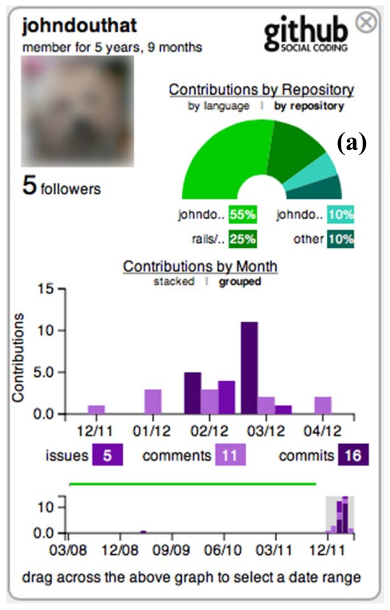
\includegraphics[width=5.0cm]{contributions.png}

\rulemajor{Rule 3: Develop forms of Legitimate Peripheral Participation}

Legitimate peripheral participation(LPP) provides newcomers with opportunities to ease into the platform and learn the norms of the community through low-risk tasks. That is, tasks that will not interrupt the community’s utility. In order to provide successful LPP newcomers with an opportunity to engage that adds value to the community. Likewise, in communities, such as GitHub, commiting code and submitting pull request to a community are the main interactions on engaging. However, these tasks can be socially daunting for newcomers~\cite{steinmacher2015social}. One form of encouraging LPP on this platform could be to encourage newcomers to add an issue to a repository when they notice a bug. Another form of LPP would be to join the dialogue on a recently submitted pull request. These provide newcomers interactive opportunities to learn the norms of the community. 

Building multiple ways of participating in a community demonstrates the variety of approaches newcomers can take to join the community. This further demonstrates that there’s not just one way to make technical contributions.  Take Stack Overflow for instance, the main form of interaction in the community is to ask a question and posting an answer. For some users, engaging in that type of interaction can present barriers including an \emph{Intimidating Community Size} and \emph{Fear of Negative Feedback}~\cite{ford2016paradise}. Thus, it is important to provide additional forms of participation. On Stack Overflow this is demonstrated through the ability to edit questions and answer without the restriction of reputation points.  Developing pathway to participation can decrease the presence of barriers. In studying the evolution of how content is formed in these communities~\cite{baltes2018evolution}, newcomers can better understand the norms of a community and the best way to contribute~\cite{ford2018wedont}.

\rulemajor{Rule 4}

\rulemajor{Rule 5}

\rulemajor{Rule 6}

\rulemajor{Rule 7: Provide an easy, complete, and up-to-date guide to contributing.}

For any form of organized activity,
it is likely more constructive and efficient to teach and reward desired behaviors
than to change problematic behaviors down the line.
Project decision-makers can prompt desired practices in open source software development
by providing newcomers with ``how to contribute'' guidelines in easy-to-find, readily-available places.
Many projects follow GitHub's recommendation for placing such information
in a CONTRIBUTING.md file (https://help.github.com/articles/setting-guidelines-for-repository-contributors/).
Other projects,
such as the Apache Open Office Suite (https://openoffice.apache.org/orientation/intro-contributing.html)
and rOpenSci (https://ropensci.github.io/dev\_guide/, Chapter 14: Contributing Guide),
provide text-based newcomer manuals and learning modules accessed through a web interface.
Still others take a more interactive approach,
such as the GNOME project's Newcomers Guide (https://wiki.gnome.org/Newcomers/SubmitContribution),
which walks potential contributors through the contribution pipeline:
choosing a project,
acquiring and installing the necessary computing tools,
finding problems or choosing issues to work on,
submitting changes,
and following up on feedback.

``How to contribute'' guidelines,
no matter the form of presentation,
serve several additional purposes alongside describing expected contribution behaviors.
Contribution guidelines offer a centralized, well-organized description of resources
that a newcomer can consult while learning to navigate the project's technical and social environments \cite{b:zanatta2017}.
Indeed, the social environment is a key constraint on newcomer behaviors \cite{b:steinmacher};
explicitly-stated definitions of contribution expectations can ease newcomers' hesitancies
about whether or not their work is sufficient and suitable for the project.
Relatedly,
guidelines also acclimate newcomers to the norms of work and communication,
particularly when items such as necessary computing tools and codes of conduct are foregrounded.
In sum,
when combined with a welcoming, inclusive environment,
clear expectations about legitimate participation,
and shared software development goals,
contribution guidelines can help newcomers feel they are on equal footing with veteran project members.

Project decision-makers should keep in mind,
though,
that their perceptions of what constitutes clear, easy-to-find contribution guidelines
may not align with the perceptions of the newcomers themselves.
Continual reevaluation of the guidelines based on community member feedback is essential
to ensuring that contribution guidelines are achieving desired effects
and do not fall out of date (e.g., as technical and social elements of the community change).
In this sense,
contribution guidelines should be treated as living, evolving documents rather than immutable rules.

\rulemajor{Rule 8}

\rulemajor{Rule 9: Keep your house in order.}

There is no point in inviting people to be a part of a dysfunctional or toxic community,
nor is there any point in making such a community more accessible or participatory,
if your goals are to grow your community and increase involvement in your project.
Likewise,
the work of creating a code of conduct will be wasted
if the enforcement process is seen to be toothless or selective.

Whatever our intentions,
our commitment to our goals and values is seen through our actions.
If new participants to our community are disciplined for the same behavior
for which longtime participants get a pass,
then you should expect any community-building efforts to fail.

\rulemajor{Rule 10: follow up on success.}

Once a new contributor has been able to carry their first contribution over the line, 
you're likely to have have a sense of their strenghts and weakensses,
and this is a good time to invite them to continue their involvement in your project.

The first and most important thing is to thank them for their contribution.
Gratitude and recognition are the most powerful tools available for community builders and maintainers. 

After that,
consider what you've learned of this contributor to help them find
the next issue they might want to work on.
If we have aspirations for our open source projects as a welcome and empopwering community,
it's important that this be an invitation,
not a suggestion or demand. 

\section*{Conclusion}

\bibliography{rules}

\end{document}
